\begin{figure}
  \centering
  \begin{tikzpicture}
    \node at (0,2.5) {$Q = 2$};
    \node at (0,0) {\includegraphics[width=3cm]{experiments/2d/ppca_occ/easy_2/results}};
    \node at (0,-3.25) {\includegraphics[width=3cm]{experiments/2d/ppca_occ/easy_2/random2}};
    \draw[-,dashed] (1.625, -4.75) -- (1.625, 2.5);
    
    \node at (3.25,2.5) {$Q = 5$};
    \node at (3.25,0) {\includegraphics[width=3cm]{experiments/2d/ppca_occ/easy_5/results}};
    \node at (3.25,-3.25) {\includegraphics[width=3cm]{experiments/2d/ppca_occ/easy_5/random2}};
    \draw[-,dashed] (3.25 + 1.625, -4.75) -- (3.25 + 1.625, 2.5);
    
    \node at (6.5,2.5) {$Q = 10$};
    \node at (6.5,0) {\includegraphics[width=3cm]{experiments/2d/ppca_occ/easy_10/results}};
    \node at (6.5,-3.25) {\includegraphics[width=3cm]{experiments/2d/ppca_occ/easy_10/random2}};
    \draw[-,dashed] (6.55 + 1.625, -4.75) -- (6.5 + 1.625, 2.5);
    
    \node at (9.75,2.5) {$Q = 25$};
    \node at (9.75,0) {\includegraphics[width=3cm]{experiments/2d/ppca_occ/easy_25/results}};
    \node at (9.75,-3.25) {\includegraphics[width=3cm]{experiments/2d/ppca_occ/easy_25/random2}};
    \node at (11.75,-1.1) {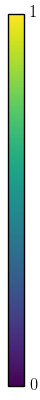
\includegraphics[height=6.8cm]{experiments/2d/ppca_occ/colorbar2}};
  \end{tikzpicture}
  % TODO short caption
  \caption{Qualitative results for \PPCA with different sizes $Q \in \{2,5,10,25\}$
  of the latent space. From top to down, we show the input shape,
  the reconstruction, the corresponding error and the thresholded reconstruction.
  The last two rows show random samples. We clipped the visualization
  to $[0, 1]$ for convenience.}
  \label{fig:experiments-2d-ppca-qual}
\end{figure}
